\section{Introduction to Calculus}

    \subsection{Limits}
        \color{purple} \textbf{The Epsilon-Delta ($\epsilon-\delta$) Definition of Limits:}
        \color{black} \\

        \noindent Let $f$ be a real-valued function, defined around around $a$.
        Then the \textbf{limit}, $L$, as $f(x)$ approaches $a$, or \textbf{converges} to $a$, is \\

        \begin{equation*}
            \lim_{x \to a} f(x) = L
        \end{equation*}

        \noindent If, $\forall \epsilon > 0$, there exists $\delta > 0$ such that if $x$ is
        within $\delta$ of $a$ (with $x\not = a$), then $f(x)$ is within $\epsilon$ of $L$.
        In other words, \\

        \begin{equation*}
            \text{If } 0 < |x-a| < \delta, \text{ then } |f(x)-L| < \epsilon
        \end{equation*}

        \begin{figure} [hbt!]
            \centering
            \begin{subfigure}[b]{.45\textwidth}
                \includegraphics{Resources/Unit1Limits/limit1.PNG}
            \end{subfigure}
            \begin{subfigure}[b]{.45\textwidth}
                \includegraphics{Resources/Unit1Limits/limit2.PNG}
            \end{subfigure}
        \end{figure}

        \noindent It is easiest to think of the limit of a function at a certain point, $a$,
        as the value of the function near $a$. For a limit, $L$, to exist at $a$, the
        \textbf{right-hand limit ($a^+$)} and the \textbf{left-hand limit ($a^-$)} must be equal. \\

        \begin{equation*}
            \lim_{x \to a} f(x) = L \implies \lim_{x \to a^+} f(x) = L = \lim_{x \to a^-} f(x)
        \end{equation*}

        \noindent \color{blue} \textit{Example 1: Find $\lim_{x\to 4}f(x)$, where the function
        $f(x)$ is given by the graph}. \color{black} \\

        \begin{center}
            \begin{tikzpicture}
                \begin{axis}[
                    axis lines = center,
                    axis equal image,
                    xmin = -3,
                    xmax = 7,
                    ymin = -3,
                    ymax = 7,
                ]
                %f(x)
                \addplot [
                    samples = 200,
                    color = red,
                ]
                {(x-2)^2-1};
                \addlegendentry{$f(x)$}
                \end{axis}
            \end{tikzpicture}
        \end{center}

        \begin{equation*}
            \lim_{x\to4^+}f(x) = 2 = \lim_{x\to4^-} f(x) \\
        \end{equation*}
        \begin{equation*}
            \therefore \lim_{x\to4} f(x) = 2
        \end{equation*}

        \noindent \color{blue} \textit{Example 2: Determine $\lim_{x\to 1} g(x)$, where the
        function $g(x)$ is graphed below. It is given that $g(x)$ is defined for all real numbers
        except $x=1$ and the graph of $g(x)$ is divided by the asymptote $x=1$.} \color{black} \\

        \begin{center}
            \begin{tikzpicture} [scale=0.75]
                \begin{axis}[
                    axis lines = center,
                    xmin = -20,
                    xmax = 20,
                    ymin = -20,
                    ymax = 20
                ]
                %g(x)
                \addplot [
                    unbounded coords=jump,
                    domain=-20:-2,
                    samples=41,
                    color=blue
                ]
                {(3*x+6)/(x-1)};
                \addlegendentry{$g(x)$}
                \addplot [unbounded coords=jump,
                    domain=-2:1,
                    samples=16,
                    color=blue,
                ]
                {(3*x+6)/(x-1)};
                \addplot [unbounded coords=jump,
                    domain=1:20,
                    samples=46,
                    color=blue,
                ]
                {(3*x+6)/(x-1)};
                %Vertical Asymptote
                \draw[dashed] (1,\pgfkeysvalueof{/pgfplots/ymin}) --
                (1,\pgfkeysvalueof{/pgfplots/ymax})
                (\pgfkeysvalueof{/pgfplots/xmin},3) --
                (\pgfkeysvalueof{/pgfplots/xmax},3);
                \end{axis}
            \end{tikzpicture}
        \end{center}

        \begin{equation*}
            \lim_{x\to 1^+}g(x) = \infty
        \end{equation*}
        \noindent and
        \begin{equation*}
            \lim_{x\to 1^-}g(x) = -\infty
        \end{equation*}

        \noindent Since the right-hand and left-hand limits do not equal each other,
        $\lim_{x\to1}g(x)$ does not exist.



    \subsection{Limit Properties}
        Assume $\lim_{x\to a}f(x)$ and $\lim_{x\to a}g(x)$ exist and that $c$ is any constant.
        Then the following properties hold true. \\

        \begin{center}
            \begin{tabular}{|c|c|}
                \hline
                $\lim_{x\to a} c=c$ & \textbf{Limit of a Constant} \\
                \hline
                $\lim_{x\to a} [cf(x)]=c\lim_{x\to a} f(x)$ & \textbf{Constant Multiple} \\
                \hline
                $\lim_{x\to a} [f(x)\pm g(x)=\lim_{x\to a}f(x)\pm\lim_{x\to a} g(x)]$ & \textbf{Sum/Difference} \\
                \hline
                $\lim{x\to a}[f(x)g(x)]=\lim_{x\to a}f(x)\lim_{x\to a}g(x)$ & \textbf{Product} \\
                \hline
                $\lim_{x\to c}(f(g(x)))=f\left(\lim_{x\to c}g(x)\right)$ &
                \textbf{Composition} \\
                \hline
                $\lim_{x\to a} \left[\frac{f(x)}{g(x)}\right]=\frac{\lim_{x\to a}f(x)}{\lim_{x\to a}g(x)}, \lim_{x\to a}g(x)\not = 0$. & \textbf{Quotient} \\
                \hline
                $\lim_{x\to a}[f(x)]^n=\left[\lim_{x\to a}f(x)\right]^n, n\in \mathbb{R}$ & \textbf{Exponent} \\
                \hline
                $\lim_{x\to a}\sqrt[3]{f(x)}\sqrt[n]{\lim_{x\to a}[f(x)]}$ & \textbf{Root} \\ \hline
                $\lim_{x\to a}x=a$ & \textbf{Limit of a Variable} \\
                \hline
            \end{tabular}
        \end{center}



    \subsection{Finding Limits from Tables}
        Tables should always be the last resort when attempting to determine limits, because
        of their tendency to be tedious. \\

        \noindent \color{blue} \textit{Example: The function $g$ is defined over the real numbers.
        This table gives a few values of $g$ What is a reasonable estimate for $\lim_{x\to 4}g(x)$?}
        \color{black} \\

        \begin{tabular}{ccccccc}
            $x$ & 3.9 & 3.99 & 3.999 & 4.001 & 4.01 & 4.1 \\
            \hline
            $g(x)$ & 11.21 & 11.92 & 11.99 & 12.01 & 12.08 & 12.81
        \end{tabular}

        \noindent $lim_{x\to 4}g(x)$ represents the limit of $g$ as $x$ approaches
        4. Looking over the table, we see that the left-hand limit appears to approach 12 as
        $x$ gets progressively larger. \\

        \begin{tabular}{cccc}
            $x$ & 3.9 & 3.99 & 3.999 \\
            \hline
            $g(x)$ & 11.21 & 11.92 & 11.99
        \end{tabular}

        \noindent We also see that the right-hand limit appears to approach 12 as $x$ gets
        progressively smaller. \\

        \begin{tabular}{cccc}
            $x$ & 4.001 & 4.01 & 4.1 \\
            \hline
            $g(x)$ & 12.01 & 12.08 & 12.81
        \end{tabular}

        \noindent Since the right-hand and left-hand limits are equal, we can conclude
        that $\lim_{x\to 4}g(x)=12$.



    \subsection{Evaluating Limits Algebraically}
        \color{purple} \textbf{The 3 Main Algebraic Limit Strategies:} \color{black} \\
        \noindent \color{purple} \textbf{1. Factoring} \color{blue} \\
        \textit{Example: Determine the limit} \color{black} \\

        \begin{align*}
            \lim_{x\to -1}\frac{x^2-x-2}{x^2-2x-3} &= \lim_{x\to -1}\frac{(x+1)(x-2)}{(x+1)(x-3)} \\
            &= \lim_{x\to -1}\frac{x-2}{x-3} \\
            &= \frac{-1-2}{-1-3} \\
            &= \frac{3}{4}
        \end{align*}

        \noindent \color{purple} \textbf{2. Conjugates} \color{blue} \\
        \textit{Example: Determine the limit} \color{black} \\
        \begin{align*}
            \lim_{x\to 4}\frac{\sqrt{x}-2}{x-4}
            &= \lim_{x\to 4}\frac{\sqrt{x}-2}{x-4}\cdot\frac{\sqrt{x}+2}{\sqrt{x}+2} \\
            &= \lim_{x\to 4}\frac{1}{\sqrt{x}+2} \\
            &= \frac{1}{4}
        \end{align*}

        \pagebreak
        \noindent \color{purple} \textbf{3. Trig Identities} \color{blue} \\
        \textit{Example: Determine the limit} \color{black} \\
        \begin{align*}
            \lim_{x\to 0} \frac{\sin{(x)}}{\sin{(2x)}}
            &= \lim_{x\to 0} \frac{\sin{(x)}}{2\sin{(x)}\cos{(x)}} \\
            &= \lim_{x\to 0} \frac{1}{2\cos{(x)}} \\
            &= \frac{1}{2}
        \end{align*}



    \subsection{Asymptotes}
        \color{purple} \textbf{Horizontal Asymptotes:} \color{black} \\
        \noindent The line $y=b$ is a \textit{horizontal asymptote} of the graph of $y=f(x)$ if \\

        \begin{equation*}
            \lim_{x\to\infty}f(x)=b\text{ or }\lim_{x\to-\infty}f(x)=b
        \end{equation*}

        \noindent It is important to note that horizontal and slant asymptotes \textit{can} be crossed,
        as they describe the general behavior of the functions as they near the edges of the graph.
        On the other hand, vertical asymptotes cannot be crossed as they describe particular
        behavior of the function itself, rather than the edges of the graph. Below is an example
        of a horizontal asymptote being crossed. \\

        \begin{center}
            \begin{tikzpicture}
                \begin{axis}[
                    axis lines = center,
                    xmin = -10,
                    xmax = 15,
                    ymin = -3,
                    ymax = 6,
                    xlabel={$x$},
                    ylabel={$y$},
                ]
                %f(x)
                \addplot [
                    domain=-10:15,
                    samples=100,
                    color=red
                ]
                {(3*x^2-8*x+7)/(x^2-4*x+5)};
                \addlegendentry{$f(x)=\frac{3x^2-8x+7}{x^2-4x+5}$}
                %asymptote
                \draw[
                    dashed
                ]
                (-10,3) -- (15,3);
                \end{axis}
            \end{tikzpicture}
        \end{center}

        \noindent \color{purple} \textbf{Vertical Asymptotes:} \color{black} \\
        The line $x=a$ is a \textit{vertical asymptote} of the graph of $y=f(x)$ if at least one
        of the below expressions holds. \\

        \begin{equation*}
            \lim_{x\to a^-}f(x)=\pm\infty,
            \lim_{x\to a^+}f(x)=\pm\infty
        \end{equation*}

        \noindent Example of a graph containing a vertical asymptote: \\

        \begin{center}
            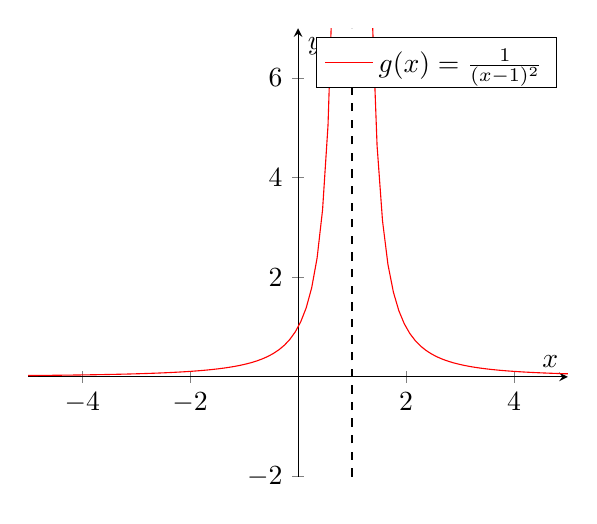
\begin{tikzpicture}
                \begin{axis}[
                    axis lines = center,
                    xmin = -5,
                    xmax = 5,
                    ymin = -2,
                    ymax = 7,
                    xlabel={$x$},
                    ylabel={$y$},
                ]
                %g(x)
                \addplot [
                    domain=-5:5,
                    samples=100,
                    color=red
                ]
                {(1)/((x-1)^2)};
                \addlegendentry{$g(x)=\frac{1}{(x-1)^2}$}
                %asymptote
                \draw[
                    dashed
                ]
                (1,-2) -- (1,7);
                \end{axis}
            \end{tikzpicture}
        \end{center}

        \noindent \color{purple} \textbf{The Rational Function Theorem:} \color{black} \\
        \noindent When $\lim_{x\to\pm\infty}\frac{P(x)}{Q(x)}=0$, $y=0$ is a horizontal asymptote
        of the graph of $y=\frac{P(x)}{Q(s)}$. \\
        When $\lim_{x\to\pm\infty}\frac{P(x)}{Q(x)}=\pm\infty$, the graph of $y=\frac{P(x)}{Q(x)}$
        has no horizontal asymptotes. \\
        When $\lim_{x\to\pm\infty}\frac{P(x)}{Q(x)}=\frac{a_n}{b_n}$, $y=\frac{a_n}{b_n}$ is a
        horizontal asymptote of the graph of $y=\frac{P(x)}{Q(x)}$.

    \pagebreak
    \subsection{The Squeeze Theorem}
        Functions $g$ and $h$ are strategically chosen to satisfy the conditions outlined in the
        definition. Notice how, in the figure after the definition, function $f$ is being
        "squeezed" between functions $g$ and $h$, hence the name. \\

        \noindent \color{purple} \textbf{The Squeeze Theorem:} \color{black} \\
        Assume that functions $f,g,h$ defined n $D\subseteq\mathbb{R}$ satisfy \\

        \begin{equation*}
            g(x)\leq f(x)\leq h(x),\forall x\in D
        \end{equation*}

        \noindent If $\lim_{x\to a}g(x)=\lim_{x\to a}h(x)=L$, then $\lim_{x\to a}f(x)=L$. \\

        \begin{center}
            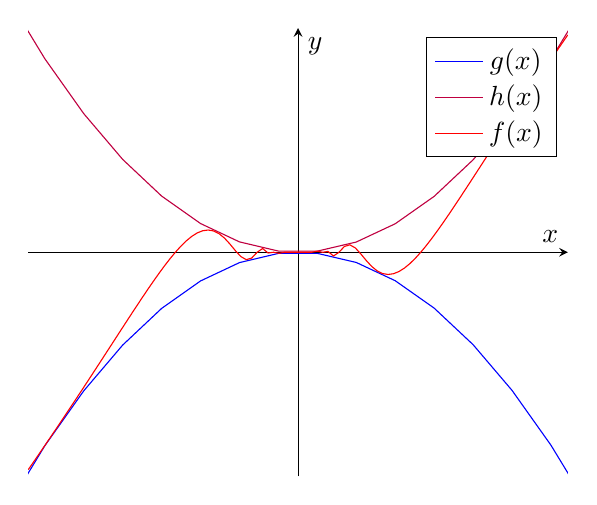
\begin{tikzpicture}
                \begin{axis}[
                    axis lines = center,
                    xmin = -0.7,
                    xmax = 0.7,
                    ymin = -0.5,
                    ymax = 0.5,
                    xlabel={$x$},
                    ylabel={$y$},
                    \pgfplotset{ticks=none}
                ]
                    %g(x)
                    \addplot [
                        samples=100,
                        color=blue
                    ]
                    {-x^2};
                    \addlegendentry{$g(x)$}
                    %h(x)
                    \addplot[
                        samples=100,
                        color=purple
                    ]
                    {x^2};
                    \addlegendentry{$h(x)$}
                    %f(x)
                    \addplot[
                        domain=-0.7:0.7,
                        samples=100,
                        color=red
                    ]
                    {x^2*sin(deg(1/\x))};
                    \addlegendentry{$f(x)$}
                \end{axis}
            \end{tikzpicture}
        \end{center}

        \noindent \color{blue}
        \textit{Example 1: Given an infinite sequence $\{a_n\}$ that satisfies
        $\frac{2n^2-7}{4n+5}<a_n<\frac{3n^2+8}{6n-1}$ for all positive integers $n$, evaluate} \\

        \begin{equation}
            \lim_{n\to \infty}\frac{3na_n}{(n+1)^2}
        \end{equation}

        \color{black} \noindent We transform the middle term of the inequality to the desired
        expression through manipulating each side of the inequality. Then the inequality becomes \\

        \begin{equation*}
            \frac{3n}{(n+1)^2}\cdot\frac{2n^2-7}{4n+5}<\frac{3na_n}{(n+1)^2}<\frac{3n}{(n+1)^2}\cdot\frac{3n^2+8}{6n-1}
        \end{equation*}

        \noindent Now we can take the limits of the top and bottom functions. \\

        \begin{align*}
            \lim_{n\to \infty}\frac{3n(2n^2-7)}{(4n+5)(n+1)^2} &= \frac{3}{2} \\
            \lim_{n\to\infty}\frac{3n(3n^2+8)}{(6n-1)(n+1)^2} &= \frac{3}{2}
        \end{align*}

        \noindent Since the top and bottom functions are equal, we can conclude that \\

        \begin{equation*}
            \lim_{n\to\infty} \frac{3na_n}{(n+1)^2}=\frac{3}{2}
        \end{equation*}

        \noindent \color{blue} \textit{Example 2: Evaluate the limit} \\

        \begin{equation*}
            \lim_{n\to\infty}\sqrt[n]{3^n+\{2|\sin{(n^n)}\}^n}
        \end{equation*}

        \color{black} \noindent We can note that \\

        \begin{equation*}
            0\leq|\sin{(n^n)}|\leq1
        \end{equation*}

        \noindent Then we can write \\

        \begin{equation*}
            \sqrt[n]{3^n}\leq\sqrt[n]{3^n+\{2|\sin{(n^n)}\}^n}\leq\sqrt[n]{3^n+2^n}\leq\sqrt[n]{2\cdot3^n}
        \end{equation*}

        \noindent The left side reduces to 3, whereas the right side becomes \\

        \begin{equation*}
            \lim_{n\to\infty}\sqrt[n]{2\cdot3^n} = 3\lim_{n\to\infty}\sqrt[n]{2}=3
        \end{equation*}

        \noindent Thus we can conclude that \\

        \begin{equation*}
            \lim_{n\to\infty} \sqrt[n]{3^n+\{2|\sin{(n^n)}|\}^n} = 3
        \end{equation*}

        \noindent \color{blue} \textit{Example 3: Evaluate the limit} \\
        \begin{equation*}
            \lim_{x\to\infty}\frac{\sin{x}}{x}
        \end{equation*} \color{black}

        \noindent Since $\forall x,-1\leq\sin{x}\leq1$, it follows that if $x>0$ then
        $-\frac{1}{x}\leq\frac{\sin{x}}{x}\leq\frac{1}{x}$. As $x\rightarrow\infty$,
        $-\frac{1}{x}$ and $\frac{1}{x}$ both approach 0. Therefore, by the Squeeze Theorem,
        $\frac{\sin{x}}{x}$ also approaches 0. \\



    \subsection{Limit of a Quotient of Polynomials}
        For the function $f(x)=\frac{P(x)}{Q(x)}$, where $P(x)$ is a polynomial of degree $n$
        and $Q(x)$ is a polynomial of degree $m$, the following expressions hold. Let $a_n$
        and $b_n$ be the leading coefficients of $P(x)$ and $Q(x)$ respectively. Then \\

        \begin{equation*}
            \text{If $n>m$, then }\lim_{x\to\infty}f(x)=\infty\text{ and }
            \lim_{x\to-\infty}f(x)=-\infty
        \end{equation*}

        \begin{equation*}
            \text{If $n=m$, then }\lim_{x\to\pm\infty}f(x)=\frac{a_n}{b_m}
        \end{equation*}

        \begin{equation*}
            \text{If $n<m$, then }\lim_{x\to\pm\infty}f(x)=0
        \end{equation*}

        \noindent This method is a shortcut found through dividing each of the terms of $P(x)$
        and $Q(x)$ by the highest power of $x$ found in $f(x)$, then taking the individual limits
        of each separated term through basic limit properties. For example, see below. \\

        \noindent \color{blue} \textit{Example: Evaluate the limit} \color{black} \\

        \begin{align*}
            \lim_{x\to\infty}\frac{x^3-4x^2+7}{3-6x-2x^3} &=
            \lim_{x\to\infty}\frac{1-\frac{4}{x}+\frac{7}{x^3}}{\frac{3}{x^3}-\frac{6}{x^2}-2} \\
            &= \frac{\lim_{x\to\infty}(1)-\lim_{x\to\infty}\left(\frac{4}{x}\right)+\lim_{x\to\infty}\left(\frac{7}{x^3}\right)}{\lim_{x\to\infty\left(\frac{3}{x^3}\right)}-\lim_{x\to\infty}\left(\frac{6}{x^2}\right)-\lim_{x\to\infty}(2)} \\
            &= \frac{1-0+0}{0-0-2} \\
            &= -\frac{1}{2}
        \end{align*}

        \noindent Note that in this case, $n=m$, so $\frac{a_n}{b_n}\implies -\frac{1}{2}$.
        Since the properties described preceding this example can be observed in all quotients
        of polynomials, we can thus make generalizations as specificed above.



    \subsection{L'Hospital's Rule}
        \textbf{L'Hospital's} is a method of evaluating limits of indeterminate forms, learned
        after gaining knowledge of derivatives. \textbf{Indeterminate forms} are expressions i
        nvolving two functions whose limits cannot be determined solely from the limits of the
        individual functions. \\

        \noindent \color{purple} \textbf{The 7 Indeterminate Forms:} \\ \color{black}

        \begin{equation*}
            \frac{0}{0}, \frac{\infty}{\infty}, 0\cdot\infty, \infty-\infty, 0^0, 1^\infty, \infty^0
        \end{equation*}

        \noindent \color{purple} \textbf{L'Hospital's Rule:} \color{black} \\
        Suppose that we have either of the cases below \\

        \begin{equation*}
            \lim_{x\to a}\frac{f(x)}{g(x)}=\frac{0}{0}, \lim_{x\to a}\frac{f(x)}{g(x)}=\frac{\pm\infty}{\pm\infty}
        \end{equation*}

        \noindent where $a\in\mathbb{R}, \infty$ or $-\infty$. Then \\

        \begin{equation*}
            \lim_{x\to a}\frac{f(x)}{g(x)}=\lim_{x\to a}\frac{f'(x)}{g'(x)}
        \end{equation*}

        \noindent \color{blue} \textit{Example 1: Evaluate the limit} \\

        \begin{equation*}
            \lim_{t\to 1}\frac{5t^4-4t^2-1}{10-t-9t^3}
        \end{equation*}
        \color{black} We have an $\frac{0}{0}$ indeterminate form here, so we use L'Hospital's to get \\

        \begin{equation}
            \lim_{t\to 1}\frac{5t^4-4t^2-1}{10-t-9t^3}=\lim_{t\to 1}\frac{20t^3-8t}{-1-27t^2}
            =\frac{20-8}{-1-27}=-\frac{3}{7}
        \end{equation}

        \noindent \color{blue} \textit{Example 2: Evaluate the limit} \\

        \begin{equation*}
            \lim_{x\to-\infty}xe^x
        \end{equation*}
        \color{black} This expression is in the form $(\infty)(0)$, meaning we will have to write
        the expression as a quotient. We know that $\frac{1}{e^x}=e^{-x}$, so we can rewrite the
        limit as \\

        \begin{equation*}
            \lim_{x\to-\infty}xe^x=\lim_{x\to-\infty}\frac{x}{e^-x}=\lim_{x\to-\infty} \frac{1}{-e^-x}=0
        \end{equation*}

        \noindent \color{blue} \textit{Example 3: Evaluate the limit} \\

        \begin{equation*}
            \lim_{x\to\infty}x^{\frac{1}{x}}
        \end{equation*} \color{black}

        \noindent This limit is of the form $\infty^0$, so we have to rewrite this expression as a different
        limit. Let \\

        \begin{equation*}
            y &= x^{\frac{1}{x}} \\
        \end{equation*}

        \noindent Since \\

        \begin{equation*}
            e^{\ln{(y)}}=y
        \end{equation*}

        \noindent we can rewrite our limit as \\

        \begin{align*}
            \lim_{x\to\infty}x^{\frac{1}{x}} &= \lim_{x\to\infty} y \\
            &= \lim_{x\to\infty}e^{\ln{(y)}} \\
            &= e^{\lim_{x\to\infty}\ln{(y)}} \\
            &= e^0 \\
            &= 1
        \end{align*}

        \noindent L'Hospital's can help us prove \textbf{the basic trig limit}, useful for
        evaluating many trig limits. \\

        \begin{equation*}
            \lim_{\theta\to0}\frac{\sin{\theta}}{\theta}=1 \text{ if $\theta$ is measured in radians}
        \end{equation*}



    \pagebreak
    \subsection{Limit Strategies}
        KhanAcademy provides a convenient flowchart to illustrate a strategy to find limits: \\

        \begin{figure} [hbt!]
            \centering
            \includegraphics[scale=0.5]{Resources/Unit1Limits/limitstrat.png}
        \end{figure}

        \noindent \color{blue} \textit{Example 1:} \color{black} \\

        \begin{align*}
            \lim_{x\to 0}\frac{\sin{3x}}{x} &= \lim_{x\to0}\frac{3\sin{3x}}{3x} \\
            &= 3\lim_{x\to0}\frac{\sin{3x}}{3x} \\
            &= 3\cdot1\\
            &= 3
        \end{align*}

        \pagebreak
        \noindent \color{blue} \textit{Example 2:} \color{black} \\

        \begin{align*}
            \lim_{x\to0}\frac{\sin{2x}}{3x} &= \frac{1}{3}\lim_{x\to0}\frac{\sin{2x}}{x}\cdot\frac{2}{2} \\
            &= \frac{2}{3}\lim_{x\to0}\frac{\sin{2x}}{2x} \\
            &=\frac{2}{3}
        \end{align*}

        \noindent \color{blue} \textit{Example 3:} \color{black} \\

        \begin{align*}
            \lim_{x\to0}\frac{|x|}{x}
        \end{align*}

        \noindent Since $|x|=x$ if $x>0$ but $|x|=-x$ if $x<0$, $\lim_{x\to 0^+}\frac{|x|}{x}
        =\lim_{x\to0^+}\frac{x}{x}=1$, whereas
        $\lim_{x\to0^-}\frac{|x|}{x}=\lim_{x\to0^-}\frac{-x}{x}=-1$.
        Since the right and left hand limits are different, we can conclude that the
        limit does not exist.

        \noindent \color{blue} \textit{Example 4:} \color{black} \\
        \begin{align*}
            \lim_{x\to\infty}\arctan{(x^3-5x+6)} &= \arctan{(\lim_{x\to\infty}x^3-5x+6)} \\
            &= \arctan{(+\infty)} \\
            &= \frac{\pi}{2}
        \end{align*}



    \subsection{Limit Definition of $e$}
        The mathematical constant $e$ is defined by \\
        \begin{equation*}
            e=\lim_{n\to\infty}\left(1+\frac{1}{n}\right)^n
        \end{equation*}



    \subsection{Continuity and Discontinuity}
        A function $f(x)$ is \textbf{continuous} at $a$ if \\

        \begin{equation*}
            \lim_{x\to a}f(x)=f(a)
        \end{equation*}

        \noindent A function $f(x)$ is \textbf{continuous over the interval} $[a,b]$ if
        $\forall a\leq x\leq b$, $x$ is continuous. A function is \textbf{discontinuous} if it
        is not continuous. \\

        \noindent \color{purple} \textbf{Common Continuous Functions:} \color{black} \\
        $\bullet$ Polynomials are continuous everywhere at a real number. \\
        $\bullet$ Rational functions are continuous at each point in their domain except where
        $Q(x)=0$. \\
        $\bullet$ The absolute value function is continuous everywhere. \\
        $\bullet$ The trigonometric, inverse trigonometric, exponential, and logarithmic functions
        are continuous everywhere. \\
        $\bullet$ Irrational functions in the form $\sqrt[n]{x}$, where $n\geq 2$, are continuous
        everywhere for which $\sqrt[n]{x}$ is defined. \\
        $\bullet$ The greatest-integer function is discontinuous at each integer. \\

        \noindent \color{purple} \textbf{Types of Discontinuities:} \\
        \noindent \textbf{Jump Discontinuity:} \color{black} \\
        In a jump discontinuity, the left and right-hand limits exist, but are different.
        For example, the graph of $y=f(x)$ below has a jump discontinuity at $x=1$. \\

        \begin{center}
            \begin{tikzpicture}
                \begin{axis}[
                    axis lines = center,
                    axis equal image,
                    xmin = -5,
                    xmax = 5,
                    ymin = -5,
                    ymax = 5,
                ]
                %f(x), x<1
                \addplot [
                    domain = -5:1,
                    samples = 100,
                    color = red
                ]
                {-x/3};
                \addlegendentry{$y=f(x)$}
                %f(x), x>1
                \addplot[
                    domain = 1:5,
                    samples = 100,
                    color = red
                ]
                {-((x-2)^2)/(2)+3.5};
                %undefined circle at x = 1
                \path[
                    draw = black,
                    fill = white,
                ]
                (1,3) circle [radius = 0.1];
                %defined circle at x = 1
                \fill[black] (1,-0.3333) circle [radius = 0.1];
                \end{axis}
            \end{tikzpicture}
        \end{center}

        \noindent \color{purple} \textbf{Removable Discontinuity:} \color{black} \\
        A function $f(x)$ has a removable discontinuity at $x=a$ if $\lim_{x\to a}f(x)$ exists,
        but either $f(a)$ does not exist or the value of $f(a)\not=\lim_{x\to a}f(x)$.
        A function with a removable discontinuity at $a$ may or may not be defined at $a$.
        For example, the graph of $y=g(x)$ below has a removable discontinuity at $x=1$.
        In this case, $g(1)=3$ instead of the limit value $\lim_{x\to1}g(x)=\sin{(1)}$. \\

        \begin{center}
            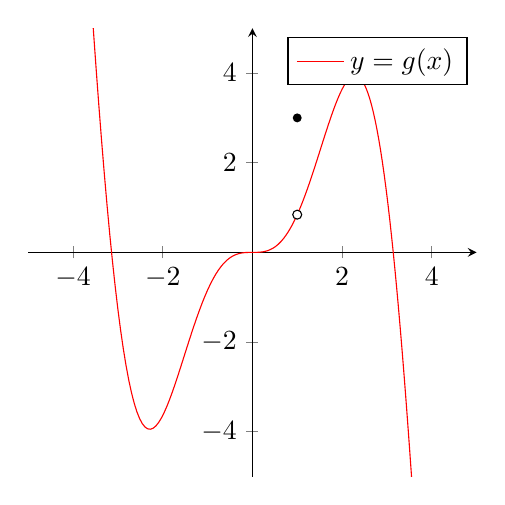
\begin{tikzpicture}
                \begin{axis}[
                    axis lines = center,
                    axis equal image,
                    xmin = -5,
                    xmax = 5,
                    ymin = -5,
                    ymax = 5,
                ]
                %g(x), x<1
                \addplot [
                    domain = -5:1,
                    samples = 100,
                    color = red
                ]
                {sin(deg(x))*x^2};
                \addlegendentry{$y=g(x)$}
                %g(x), x>1
                \addplot[
                    domain = 1:5,
                    samples = 100,
                    color = red
                ]
                {sin(deg(x))*x^2};
                %undefined circle at x = 1
                \path[
                    draw = black,
                    fill = white,
                ]
                (1,0.84147) circle [radius = 0.1];
                %defined circle at x = 1
                \fill[black] (1,3) circle [radius = 0.1];
                \end{axis}
            \end{tikzpicture}
        \end{center}

        \noindent \color{purple} \textbf{Infinite Discontinuities:} \color{black} \\
        Infinite discontinuities always occur at vertical asymptotes. There may be a vertical
        asymptote at either one or both sides of the function. An example of an infinite
        discontinuity is given below, where $y=h(x)$. \\

        \begin{center}
            \begin{tikzpicture}
                \begin{axis}[
                    axis lines = center,
                    axis equal image,
                    xmin = -5,
                    xmax = 5,
                    ymin = -3,
                    ymax = 7,
                ]
                %h(x)
                \addplot [
                    samples = 100,
                    color = red
                ]
                {1/((x-1)^2)};
                \addlegendentry{$y=h(x)$}
                %asymptote
                \draw[
                    dashed
                ]
                (1,-3) -- (1,7);
                \end{axis}
            \end{tikzpicture}
        \end{center}

        \noindent Here is an example of an \color{purple} \textbf{Infinite Oscillation Discontinuity}.
        \color{black} \\

        \begin{center}
            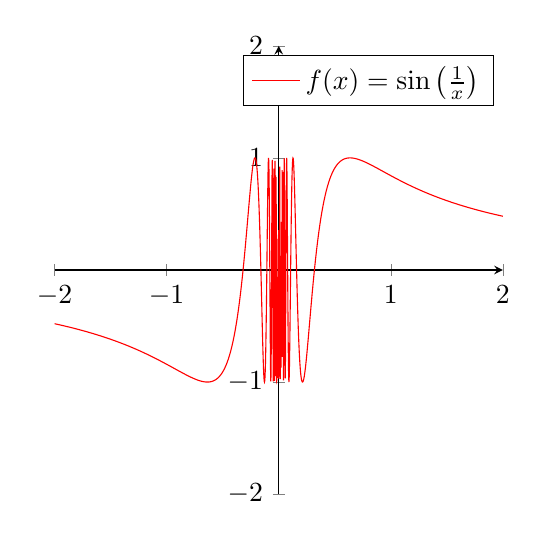
\begin{tikzpicture}
                \begin{axis}[
                    axis lines = center,
                    axis equal image,
                    xmin = -2,
                    xmax = 2,
                    ymin = -2,
                    ymax = 2,
                ]
                %f(x)
                \addplot [
                    samples = 5000,
                    color = red
                ]
                {sin(deg(1/x))};
                \addlegendentry{$f(x)=\sin{\left(\frac{1}{x}\right)}$}
                \end{axis}
            \end{tikzpicture}
        \end{center}

        \noindent \color{purple} \textbf{Essential Discontinuities} \color{black} are discontinuities
        that at which the limit of the function does not exist. Jump and infinite discontinuities
        are essential discontinuities. \\\\

        \noindent Below is a general example about continuity and discontinuity. \\
        \color{blue} \textit{Example: Is} \\

        \begin{equation*}
            f(x)=\begin{cases}
            {
            x^2+2 & x\leq 1 \\
            4 & x > 1
            }
            \end{cases}
        \end{equation*}

        \noindent continuous at $x=1$? \color{black} \\
        Since $\lim_{x\to 1^-}f(x)=3\not=\lim_{x\to 1^+}f(x)=4$.

    \subsection{The Extreme Value Theorem}
        This theorem is best learnt after derivatives. \\
        \color{purple} \textbf{The Extreme Value Theorem} \color{black} \\
        If real numbers $a$ and $b$ satisfy $a<b$ and a function $f$ is continuous on $[a,b]$,
        then $f$ attains a maximum and minimum value on $[a,b]$. \\

        \noindent \color{blue} \textit{Example: Find the maximum and minimum values of the
        function $f(x)=x^3-\frac{9}{2}x^2-12x+20$ on the interval $[-2,6]$}. \color{black} \\
        $f(x)$ is differentiable, hence continuous on the closed and bounded interval. Having
        satisfied the preconditions, we can apply the EVT to this context. Taking the first
        derivative of $f(x)$, we get \\

        \begin{align*}
            f'(x) &= 3x^2 -9x -12 \\
            &= 3(x^2-3x-4)
        \end{align*}

        \noindent Setting $f'(x)=0$ and solving, we find that the critical points are $x=-1,4$
        which by the first derivative test gives the relative extrema $y=26.5,-36$, respectively.
        Computing the endpoints, we have $f(-2)=18$ and $f(6)=2$. Hence, the minimum value of $f$
        on $[-2,6]$ is -36 and the maximum value is 26.5.



    \subsection{The Intermediate Value Theorem}
        \color{purple} \textbf{The Intermediate Value Theorem:} \color{black} \\
        If a function $f$ is continuous on the closed interval $[a,b]$, and $M$ is a number such
        that $f(a)\leq M\leq f(b)$, then there is at least one number $c$ such that $f(c)=M$. \\

        \noindent \color{blue} \textit{Example: Does a $x$ exist for some $x\in[0,2]$ such that
        the function $f(x)=x^2+\cos{(\pi x)}=4$?} \color{black} \\

        \begin{align*}
            f(0) = 0^2 + \cos{0} = 1 \\
            f(2) = 2^2 + \cos{2\pi} = 5
        \end{align*}

        \noindent Since $f(0)=1<4<5=f(2)$ and $f$ is continuous, the IVT implies that $f(x)=4$
        for some $x\in[0,2]$.



    \subsection{The Continuous Functions Theorem}
        \color{purple} \textbf{The Continuous Functions Theorem:} \color{black} \\
        If functions $f$ and $g$ are both continuous at $x=c$, then the following functions are
        also continuous: \\

        \begin{tabular}{cc}
            Constant Multiples: & $k\cdot f(x)$ for any real number $k$ \\
            Sums: & $f(x)+g(x)$ \\
            Differences: & $f(x)-g(x)$ \\
            Products: & $f(x)\cdot g(x)$ \\
            Quotients: & $\frac{f(x)}{g(x)}, g(c)\not=0$
        \end{tabular}



    \subsection{The Composition of Continuous Functions Theorem}
        \color{purple} \textbf{The Composition of Continuous Functions Theorem:} \color{black} \\
        If the function $g$ is continuous at $x=c$ and the function $f$ is continuous at $x=g(c)$,
        then the composite function $(f\circ g)(x)$ is continuous at $x=c$.